\documentclass{article}
\usepackage{tikz,amsmath,siunitx}
\usetikzlibrary{calc}
\usetikzlibrary{positioning}
\usetikzlibrary{arrows,snakes,backgrounds,patterns,matrix,shapes,fit,calc,shadows,plotmarks}
\usepackage[graphics,tightpage,active]{preview}
\PreviewEnvironment{tikzpicture}
\PreviewEnvironment{equation}
\PreviewEnvironment{equation*}
\newlength{\imagewidth}
\newlength{\imagescale}
\pagestyle{empty}
\thispagestyle{empty}
\begin{document}
\begin{tikzpicture} [auto, node distance=0 cm]
\node at (0,0) (A) {
\begin{tikzpicture}
\node[anchor=south west, inner sep=0] at (0,0) (foo) {\includegraphics[width=0.5\columnwidth]{Figures/revised_Fluidigm_Multivariate_CCR7_GZMK.pdf}};
\begin{scope} [x={(foo.south east)},y={(foo.north west)}]
\node at (0,1) [font=\tiny\sffamily] {A} ;
\end{scope}
\end{tikzpicture}
};
\node [right=of A] (B){
\begin{tikzpicture}
\node[anchor=south west, inner sep=0] at (0,0) (bar) {\includegraphics[width=0.5\columnwidth]{Figures/revised_Fluidigm_Marginal_CCR7_GZMK.pdf}};
\begin{scope} [x={(bar.south east)},y={(bar.north west)}]
\node at (-0.02,1) [font=\tiny\sffamily] {B} ;
\end{scope}
\end{tikzpicture}
};
%\node [anchor = south west, inner sep=0] at (0,-4) {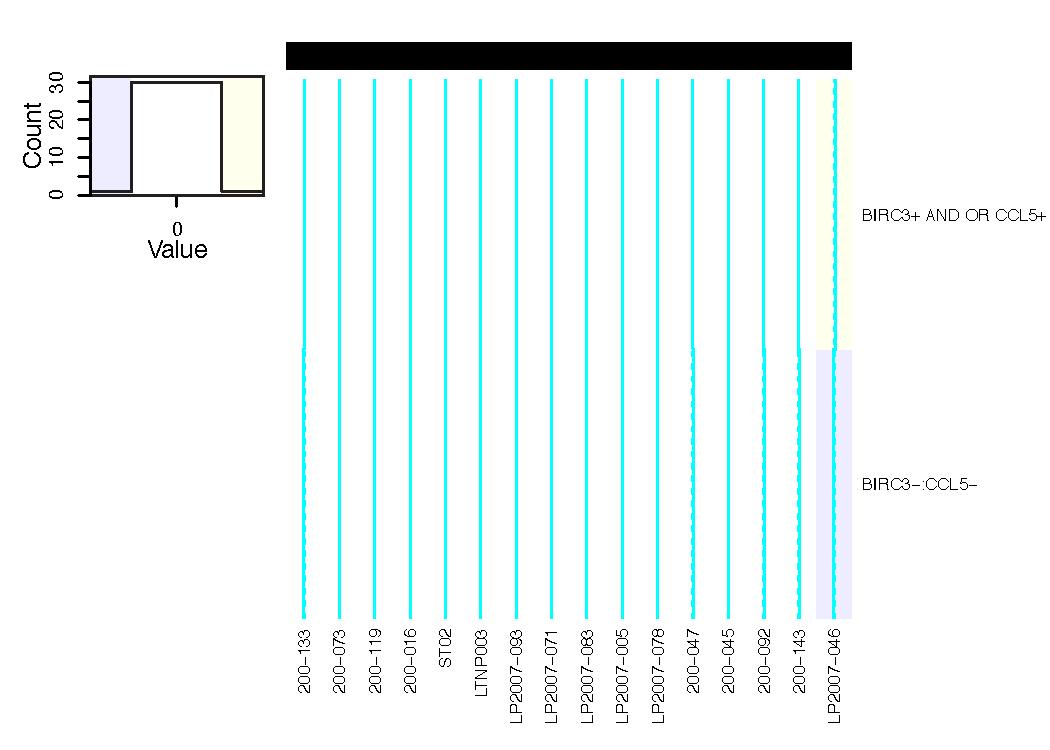
\includegraphics[width=0.4\columnwidth]{Fluidigm_Multivariate_Marginalized_BIRC3_CCL5.pdf}};
%\node [anchor=south west, inner sep=0] at (6.5,-4) {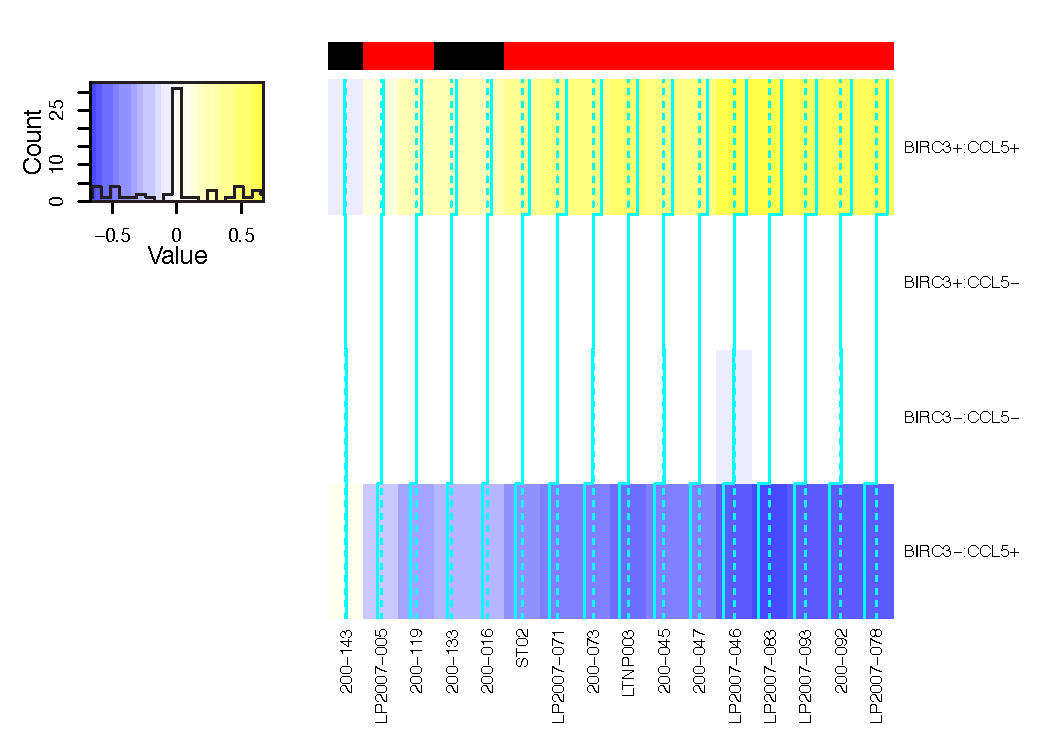
\includegraphics[width=0.4\columnwidth]{Fluidigm_Multivariate_BIRC3_CCL5.pdf}};
%\node at (0,0) [font=\small\sffamily] {C} ;
%\node at (6.25,0) [font=\small\sffamily] {D} ;
\end{tikzpicture}\end{document}
